\chapter[Transforming the Enriched Lambda Calculus][Transforming the Enriched Lambda Calculus]{Transforming the Enriched\\Lambda Calculus}
\vspace{3cm}

Having now defined the semantics of pattern-matching, we are in a position to
show how to transform all the constructs of the enriched lambda calculus into
the ordinary lambda calculus.

Section 6.1 shows how to transform pattern-matching lambda abstractions
into the ordinary lambda calculus, while Section 6.2 deals with let- and
letrec-expressions; Sections 6.3 and 6.4 deal with \ml{case}-expressions and the \fatbar{}
operator.

\section{Transforming Pattern-matching Lambda Abstractions}

In order to translate Miranda function definitions involving pattern-matching
into the enriched lambda calculus, we had to introduce pattern-matching
lambda abstractions as a new construct. In this section we will show how they
can be transformed into the ordinary lambda calculus. For each form of \ml{(\tlb{p}E)}
we will give an equivalent form that does not use pattern-matching lambda
abstractions.

In the case when the pattern \ml{p} is a variable there is nothing to do, because
no pattern-matching is involved. The remaining cases are when the pattern is
a constant, a product-constructor pattern or a sum-constructor pattern. These
are dealt with in the following three subsections.

\subsection{Constant Patterns}

This section shows how to transform a pattern-matching lambda abstraction
\ml{(\tlb{k}E)}, with a constant pattern \ml{k}, into the ordinary lambda calculus. First of
all, we recall the semantics of \ml{(\tlb{k}E)} from Section 4.3.2:

\begin{letalign}
\metafnbb{Eval}{\tlb{k}E} a = \metafnbb{Eval}{E} \qquad & \text{if} a $=$ \metafnbb{Eval}{k}\\
\metafnbb{Eval}{\tlb{k}E} a = FAIL &\text{if} a $\neq$ \metafnbb{Eval}{k}  \text{and} a $\neq \bot$  \\
\metafnbb{Eval}{\tlb{k}E} $\bot = \bot$
\end{letalign}
Operationally, \ml{(\tlb{k}E)} tests whether its argument is equal to \ml{k}; if so, it returns
\ml{E}, if not it returns \ml{FAIL}. This simple test can be carried out by the built-in \ml{IF}
function, using the following transformation:
\begin{mlcoded}
(\tlb{k}E) $\equiv$ (\tlb{v}   IF (= k v) E FAIL)
\end{mlcoded}
where \ml{v} is a new variable which does not occur free in \ml{E}. It should be clear
(and can be proved, using the semantics of  \ml{(\tlb{k}E)} and the semantics of \ml{IF} and
\ml{=}) that these two lambda abstractions have the same meaning, and hence are
equivalent. Notice the way in which we introduce a new \ml{\tl{v}} abstraction, so that
we can name the argument directly in its body.

As an example, consider the Miranda definition
\begin{mlcoded}
flip 0 = 1\\
flip 1 = 0
\end{mlcoded}
This will be translated to
\begin{mlcoded}
	\begin{tabular}{lll}
		flip = \tlb{x} &( &((\tlb{0} 1) x) \\
		& \fatbar{}  &((\tlb{1} 0) x) \\
		& \fatbar{} &ERROR)
	\end{tabular}
\end{mlcoded}
Now, transforming out the pattern-matching lambda abstractions gives
\begin{mlcoded}
	\begin{tabular}{lll}
		flip = \tlb{x} &( &((\tlb{v} IF (= 0 v) 1 FAIL) x) \\
		& \fatbar{}  &((\tlb{v} IF (= 1 v) 0 FAIL) x) \\
		& \fatbar{} &ERROR)
	\end{tabular}
\end{mlcoded}
It is now easy to verify that
\begin{mlcoded}
\begin{tabular}{llllll}
flip 0 & $\to$ & $\cdots$ & $\to$ & 1 \\
flip 1 & $\to$ & $\cdots$ & $\to$ & 0 \\
flip 2 & $\to$ & $\cdots$ & $\to$ & ERROR \\
\end{tabular}
\end{mlcoded}

\subsection{Product-constructor Patterns}

Next we consider the case of \ml{(\tlb{p}E)}, where \ml{p} is the product pattern
\ml{(t p$_1$ \ldots p$_r$)}, and \ml{t} is a product constructor of arity $r$. As before, we recall its
semantics (Section 4.3.4):
\begin{letalign}
	\metafnbb{Eval}{\tlb{(t p$_1$ $\ldots$ p$_r$)}E} a = \metafnbb{Eval}{ \tl{p$_1$} $\ldots$ \tlb{p$_r$}E } & (SEL-t-1 a)\\
	& $\cdots$\\
	& (SEL-t-r a)
\end{letalign}

To implement this semantics, we invent a new function
\ml{UNPACK-PRODUCT-t} for each product constructor \ml{t}, and use it in this
transformation:
\begin{mlcoded}
(\tlb{(t p$_1$ $\ldots$ p$_r$)}E) $\equiv$ UNPACK-PRODUCT-t (\tl{p$_1$}$\ldots$\tlb{p$_r$}E)
\end{mlcoded}
The idea is that \ml{UNPACK-PRODUCT-t} takes two arguments, a function and a
structured object, and applies the function to the lazily selected components
of the object. It is defined by the following semantic equation:
\begin{mlcoded}
UNPACK-PRODUCT-t f a $=$ f (SEL-t-1 a) $\cdots$ (SEL-t-r a)
\end{mlcoded}
It can easily be shown that the transformation is valid, by comparing the 
semantics of the expression before and after the transformation.

The right-hand side of the transformation still has pattern-matching lambda
abstractions in it, but they are smaller than the one we began with, and
repeated use of the rules for transforming pattern-matching lambda 
abstractions will eliminate them.

As an example, consider the function \ml{addPair}, which adds together the
elements of a pair:
\begin{mlcoded}
	addPair = \tlb{PAIR x y} + x y
\end{mlcoded}
This will be transformed to
\begin{mlcoded}
	addPair = UNPACK-PRODUCT-PAIR (\tlb{x}\tlb{y}+ x y)
\end{mlcoded}
We can check that it gives the right results by reducing \ml{(addPair (PAIR 3 4))}:
\begin{mlcoded}
	addPair (PAIR 3 4)\\
	\phantom{--}= UNPACK-PRODUCT-PAIR (\tlb{x}\tlb{y}+ x y) (PAIR 3 4) \\
	$\rightarrow$ (\tlb{x}\tlb{y}+ x y) (SEL-PAIR-1 (PAIR 3 4)) (SEL-PAIR-2 (PAIR 3 4)) \\ 
	$\rightarrow$ (\tlb{y}+ (SEL-PAIR-1 (PAIR 3 4)) y) (SEL-PAIR-2 (PAIR 3 4)) \\
	$\rightarrow$ + (SEL-PAIR-1 (PAIR 3 4)) (SEL-PAIR-2 (PAIR 3 4)) \\
	$\rightarrow$ + 3 (SEL-PAIR-2 (PAIR 3 4)) \\  
	$\rightarrow$ + 3 4 \\
	$\rightarrow$ 7
\end{mlcoded}

\subsection{6.1.3 Sum-constructor Patterns}

Finally, consider the case of \ml{(\tlb{p}E)}, where \ml{p} is a sum pattern \ml{(s p$_1$ $\cdots$ p$_r$)}, and
\ml{s} is a sum constructor of arity \ml{r}. The semantics of such lambda abstractions
was derived in Section 4.3.3:
\begin{letalign}
	\metafnbb{Eval}{\tlb{(s p$_1$\,\ldots\,p$_r$)}E} (s a$_1$\,\ldots\,a$_r$) 
	&= \metafnbb{Eval}{\tl{p$_1$}\ldots\tlb{p$_r$}E} a$_1$\,\ldots\,a$_r$ \\
	\metafnbb{Eval}{\tlb{(s p$_1$\,\ldots\,p$_r$)}E} (s$'$ a$_1$\,\ldots\,a$_{r'}$) 
	&= FAIL \qquad {\normalfont if} s$\,\neq\,$s$'$ \\
	\metafnbb{Eval}{\tlb{(s p$_1$\,\ldots\,p$_r$)}E} $\bot$
	&= $\bot$ \\
\end{letalign}


We can make a very similar transformation to the product-constructor case,
leaving all the hard work to a new function \ml{UNPACK-SUM-s}:
\begin{mlcoded}
	(\tlb{(s p$_1$\,\ldots\,p$_r$)}E) $=$ UNPACK-SUM-s (\tl{p$_1$}\,\ldots\,\tlb{p$_r$}E)
\end{mlcoded}

The function \ml{UNPACK-SUM-s} takes two arguments, a function (in this case
\ml{(\tl{p$_1$} \ldots \tlb{p$_r$}. E)}), and a structured object. It checks whether the object is built
with constructor \ml{s}: if not, \ml{FAIL} is returned; if so, \ml{UNPACK-SUM-s} takes the
object apart and applies the function (its first argument) to its components.
\ml{UNPACK-SUM-s} is specified by the following semantic equations:
\begin{letalign}
	UNPACK-SUM-s f (s a$_1$\,\ldots\,a$_r$) &= f\,a$_1$\,\ldots\,a$_r$ \\
	UNPACK-SUM-s f (s$'$ a$_1$\,\ldots\,a$_{r'}$) &= FAIL \qquad {\normalfont if} s\,$\neq$\,s$'$\\
	UNPACK-SUM-s f $\bot$ &= $\bot$
\end{letalign}

As an example, recall the Miranda definition of \ml{reflect}:
\begin{letalign}
	reflect (LEAF n) &= LEAF n\\
	reflect (BRANCH t$_1$ t$_2$) &= BRANCH (reflect t$_2$) (reflect t$_1$)
\end{letalign}
This is translated to:
\begin{mlalign}
	reflect = \tlb{t}&( ((\tlb{(LEAF\ n)}LEAF\ n) t)\\
	&\fatbar{} ((\tlb{(BRANCH t$_1$\ t$_2$)}BRANCH (reflect\ t$_2$) (reflect\ t$_1$)) t)\\
	&\fatbar{}  ERROR)
\end{mlalign}
Now, applying the transformation gives:
\begin{mlalign}
	reflect\\
	= \tl{t}. &( (UNPACK-SUM-LEAF (\tl{n}. LEAF\ n) t)\\
	&\fatbar{}  (UNPACK-SUM-BRANCH (\tlb{t$_1$}\tlb{t$_2$}BRANCH (reflect\ t$_2$) (reflect\ t$_1$)) t)\\
	&\fatbar{}  ERROR)
\end{mlalign}

\subsection{Reducing the Number of Built-in Functions}

The trouble with the transformations of the previous section is that they
introduce several functions associated with each constructor. In this section,
we discuss the implementation of these functions.

A structured object will be represented by the implementation as an
aggregate, consisting of the component fields together with a \textit{structure tag},
which distinguishes objects built by different constructors from each other
(see Section \ml{10.3.1}). It is this tag which can be used by \ml{UNPACK-SUM-s} to
identify the constructor used.

In a type-checked system, it is only necessary to distinguish objects from
other objects of the same type, so the structure tag can be a small integer in the
range \ml{1} \ldots \ml{n} (where \ml{n} is the number of constructors in the type). This means
that, instead of requiring an \ml{UNPACK-SUM-s} function for each constructor \ml{s},
it is only necessary to have a single family of functions \ml{UNPACK-SUM-d-r$_s$},
where \ml{d} is the integer structure tag which is recognized by \ml{UNPACK-SUM-d-r$_s$},
and \ml{r$_s$} is the arity of \ml{s}. In a similar way, the sum constructor functions can be
replaced with a family of functions \ml{PACK-SUM-d-r$_s$}, which take \ml{r$_s$} arguments
and construct an aggregate with \ml{r$_s$} fields and structure tag \ml{d}.

We can perform an analogous set of replacements for the functions
associated with product types. \ml{UNPACK-PRODUCT-t} can be replaced with
\ml{UNPACK-PRODUCT-r$_t$}, where \ml{r} is the arity of \ml{t} (there is no need for a structure
tag here, since \ml{UNPACK-PRODUCT} does not examine it). Similarly, the
product-constructor functions can be replaced with \ml{PACK-PRODUCT-r$_t$}, and
the selector functions \ml{SEL-t-i} can be replaced with \ml{SEL-r$_{t}$-i}. It is sensible to
keep \ml{PACK-SUM} and \ml{PACK-PRODUCT} distinct because, having no structure
tag, objects of product type may have a different representation from objects
of sum type.

To summarize:
\vspace{0.5\baselineskip}

{\setlength{\tabcolsep}{1pt}
\begin{tabular}{rl}
	\ml{s} (a sum-constructor function) &is replaced by \ml{PACK-SUM-d-r$_s$}\\
	\ml{UNPACK-SUM-s} &is replaced by \ml{UNPACK-SUM-d-r$_s$}\\
	\ml{t} (a product-constructor function) &is replaced by \ml{PACK-PRODUCT-r$_t$}\\
	\ml{UNPACK-PRODUCT-t} &is replaced by \ml{UNPACK-PRODUCT-r$_t$}\\
	\ml{SEL-t-i} &is replaced by \ml{SEL-r$_{t}$-i}
\end{tabular}

\begin{tabular}{rl}
where \ml{r$_s$} &$=$ arity of \ml{s},\\
\ml{d} &$=$ structure tag of \ml{s},\\
\ml{r$_t$} &$=$ arity of \ml{t}.\\
\end{tabular}
}
\vspace{0.5\baselineskip}

For example, assuming that we implement lists with structure tag $1$ for \ml{NIL}
and $2$ for \ml{CONS}, then the following replacements would take place:
\vspace{0.5\baselineskip}

{\setlength{\tabcolsep}{1pt}
	\begin{tabular}{rl}
	\ml{NIL} &is replaced by \ml{PACK-SUM-1-0}\\
	\ml{CONS} &is replaced by \ml{PACK-SUM-2-2}\\
	\ml{UNPACK-SUM-NIL} &is replaced by \ml{UNPACK-SUM-1-0}\\
	\ml{UNPACK-SUM-CONS} &is replaced by \ml{UNPACK-SUM-2-2}
\end{tabular}
}
\vspace{0.5\baselineskip}

Likewise, if the type \ml{tree} is declared as before:
\begin{mlcoded}
	tree ::= LEAF num | BRANCH tree tree
\end{mlcoded}
and \ml{LEAF} and \ml{BRANCH} are assigned structure tags 1 and 2 respectively, the
following replacements would take place:
\vspace{0.5\baselineskip}

{\setlength{\tabcolsep}{1pt}
\begin{tabular}{rl}
	\ml{LEAF} &is replaced by \ml{PACK-SUM-1-1}\\
	\ml{BRANCH} &is replaced by \ml{PACK-SUM-2-2}\\
	\ml{UNPACK-SUM-LEAF} &is replaced by \ml{UNPACK-SUM-1-1}\\
	\ml{UNPACK-SUM-BRANCH} &is replaced by \ml{UNPACK-SUM-2-2}
\end{tabular}
}\vspace{0.5\baselineskip}

Finally, if the type \ml{pair} is declared as before:
\begin{mlcoded}
	pair $*$ $**$ ::= PAIR $*$ $**$
\end{mlcoded}
the following replacements would take place:
\vspace{0.5\baselineskip}

{\setlength{\tabcolsep}{1pt}
	\begin{tabular}{rl}
	\ml{PAIR} &is replaced by \ml{PACK-PRODUCT-2}\\
	\ml{UNPACK-PRODUCT-PAIR} &is replaced by \ml{UNPACK-PRODUCT-2}\\
	\ml{SEL-PAIR-1} &is replaced by \ml{SEL-2-1}\\
	\ml{SEL-PAIR-2} &is replaced by \ml{SEL-2-2}
\end{tabular}
\vspace{0.5\baselineskip}

Since functions with different types may be replaced by the same function
(for example, \ml{CONS} and \ml{BRANCH} are both replaced by \ml{PACK-SUM-2-2}), these
replacements should not be performed until after type-checking. For the
same reason, none of these replacements is possible for a system that
performs run-time type-checking (see Section 10.5).

\subsection{Summary}
Figure 6.1 summarizes the transformations developed in this section, and
Figure 6.2 gives the semantics for the two new families of functions we
introduced in order to perform the transformations.


\boxedfigure{
	\begin{mlcoded}
	\begin{tabular}{lll}
			(\tlb{k}E)	& $\equiv$  (\tlb{v} IF (= k v) E FAIL) \\
			&  \phantom{ $\equiv$  } {\normalfont where} v {\normalfont is a new variable that does not } \\
			&	\phantom{ $\equiv$  } \qquad{\normalfont occur free in} E\\
			(\tlb{(t p$_1$ \ldots p$_{r_t}$)E}) & $\equiv$ (UNPACK-PRODUCT-t (\tlb{p$_1$ \ldots p$_{r_t}$ E})) \\
			(\tlb{(s p$_1$ \ldots p$_{r_s}$) E}) & $\equiv$ (UNPACK-SUM-s (\tlb{p$_1$ \ldots p$_{r_s}$ E}))
	\end{tabular}
	\end{mlcoded}
	
		\begin{tabular}{lll}
			where	& \ml{k}  & is a constant \\
			& \ml{t} & is a product constructor of arity \ml{r$_t$}\\
			& \ml{s} & is a sum constructor of arity \ml{r$_s$}
		\end{tabular}
}{Transforming out pattern-matching lambda abstractions}


\boxedfigure{
	\begin{mlcoded}
		UNPACK-PRODUCT-t f a = f (SEL-t-1 a) \ldots (SEL-t-r$_t$ a) \\
		
		\begin{tabular}{lll}
			UNPACK-SUM-s f (s a$_1$ \ldots a$_{r_s}$) &= f a$_1$ \ldots a$_{r_s}$ \\
			UNPACK-SUM-s f (s' a$_1$ \ldots a$_{r_{s'}}$) &= FAIL  \qquad {\normalfont if} s\,$\neq$\,s$'$\\
			UNPACK-SUM-s f $\bot$ &=$\bot$
		\end{tabular}
	\end{mlcoded}
	
	\begin{tabular}{lll}
		where & \ml{t} & is a product constructor of arity \ml{r$_t$}\\
		& \ml{s} & is a sum constructor of arity \ml{r$_s$}
	\end{tabular}
}{Semantics of \ml{UNPACK-PRODUCT} and \ml{UNPACK-SUM}}


\section{Transforming \ml{let} and \ml{letrec}}

In Section 4.2.9 we introduced a new complication to \ml{let}(\ml{rec})-expressions, by
allowing the left-hand side of definitions to be an arbitrary pattern rather than
a simple variable. In this section we show how to transform these generalized
\ml{let}s and \ml{letrec}s into successively simpler forms, arriving eventually at the
ordinary lambda calculus.

Rather than defining the semantics of \ml{let} and \ml{letrec} directly, as we did for
pattern-matching lambda abstractions, we will regard the transformations
described in this section as a definition of their semantics. To define their
meaning in a more direct way would require more mathematical machinery
than we have available in this book.

We begin by sketching a new problem which is introduced by allowing
arbitrary patterns on the left-hand side of definitions. This leads us to define a
class of patterns, the \textit{irrefutable} patterns, which do not suffer from the
problem. Then, before embarking on the transformations themselves, we
give a 'map' to explain their structure.

\subsection{Conformality Checking and Irrefutable Patterns}

Allowing arbitrary patterns on the left-hand side of a definition introduces a
new and somewhat subtle complication. Consider the expression
\begin{mlcoded}
	let (CONS x xs) = B in E
\end{mlcoded}
Here, the pattern \ml{(CONS x xs)} appears on the left-hand side of the definition.
This raises the nasty possibility that B might evaluate to \ml{NIL} instead of
\ml{(CONS B$_1$ B$_2$)}, in which case the pattern would not match, and some sort of
error should, presumably, be reported. This requires that a \textit{conformality
check} be made, to ensure that B conforms with the specified pattern.
Conformality checking will carry some implementation cost, so we would
like to avoid it whenever possible. It can be avoided in precisely those cases
when the pattern match cannot fail; for example, simple product patterns.
However, there are some nested patterns which cannot fail also, which
motivates the following definition:


\simpletitledbox{DEFINITION}{
A pattern \ml{p} is \textit{irrefutable} if it is
\begin{numbered}
	\item either a variable \ml{v}
	\item or a product pattern of form \ml{(t p$_1$ \ldots p$_{r_t}$)} where \ml{p$_1$}, \ldots, \ml{p$_{r_t}$} are irrefutable patterns.
\end{numbered}
Otherwise the pattern is \textit{refutable}.
}

\noindent In other words, the irrefutable patterns consist of arbitrarily nested product
constructors with variables at the leaves. These patterns cannot fail to match
in a type-checked implementation. Variables and simple product patterns are
just two examples of irrefutable patterns.

However, even a single constant or sum constructor (even if nested inside a
product pattern) makes the pattern refutable, since there is a possibility that it
may not match. We need to perform conformality checking for refutable
definitions only.

\subsection{Overview of let and letrec Transformations}
We are now ready to describe the various transformations to simplify \ml{let}(\ml{rec})-
expressions. While few are complicated, they are quite numerous, so we
begin by offering a `map' to aid in navigation through the rest of the section.

For a start, we establish the following terminology:
\begin{numbered}
	\item The left-hand side of each definition of a simple \ml{let(rec)}-expression must
	be a variable.
	\item The left-hand side of each definition of an irrefutable \ml{let(rec)}-expression
	must be an irrefutable pattern.
	\item The left-hand side of each definition of a general \ml{let(rec)}-expression may
	be any arbitrary pattern.
\end{numbered}
With the aid of this terminology, Figure 6.3 depicts the transformations which
will be described below, giving the appropriate section number in brackets.

For the reasons discussed in Section 3.2.4, there are two possible forms into
which we may wish to transform the program, which differ only in their
treatment of \ml{let} and \ml{letrec}:
\begin{numbered}
	\item We may transform the program into the ordinary lambda calculus; this
	gives the simplest resulting program. In this case, general \ml{let}s are trans-
	formed into the ordinary calculus via irrefutable \ml{let}s and simple \ml{let}s.
	General \ml{letrec}s, on the other hand, are first transformed into irrefutable
	\ml{let}s via irrefutable \ml{letrec}s, and then use the \ml{let} transformations.
	\item We may transform the program into the ordinary lambda calculus
	augmented with simple \ml{let(rec)}-expressions; the resulting program is
	slightly more complicated, but can be implemented more efficiently
	(Section 3.2.4). In this case, general \ml{let}s are transformed only into simple
	\ml{let}s, and general \ml{letrec}s are transformed into simple \ml{letrec}s, via irrefutable
	\ml{letrec}s.
\end{numbered}

\begin{figure}[H]
	\centering
	
	\fbox{%
		\begin{minipage}{0.9\textwidth}
			\small
			\setlength{\parindent}{10pt}
			\setlength{\parskip}{0mm plus 0mm minus 0mm}
			
			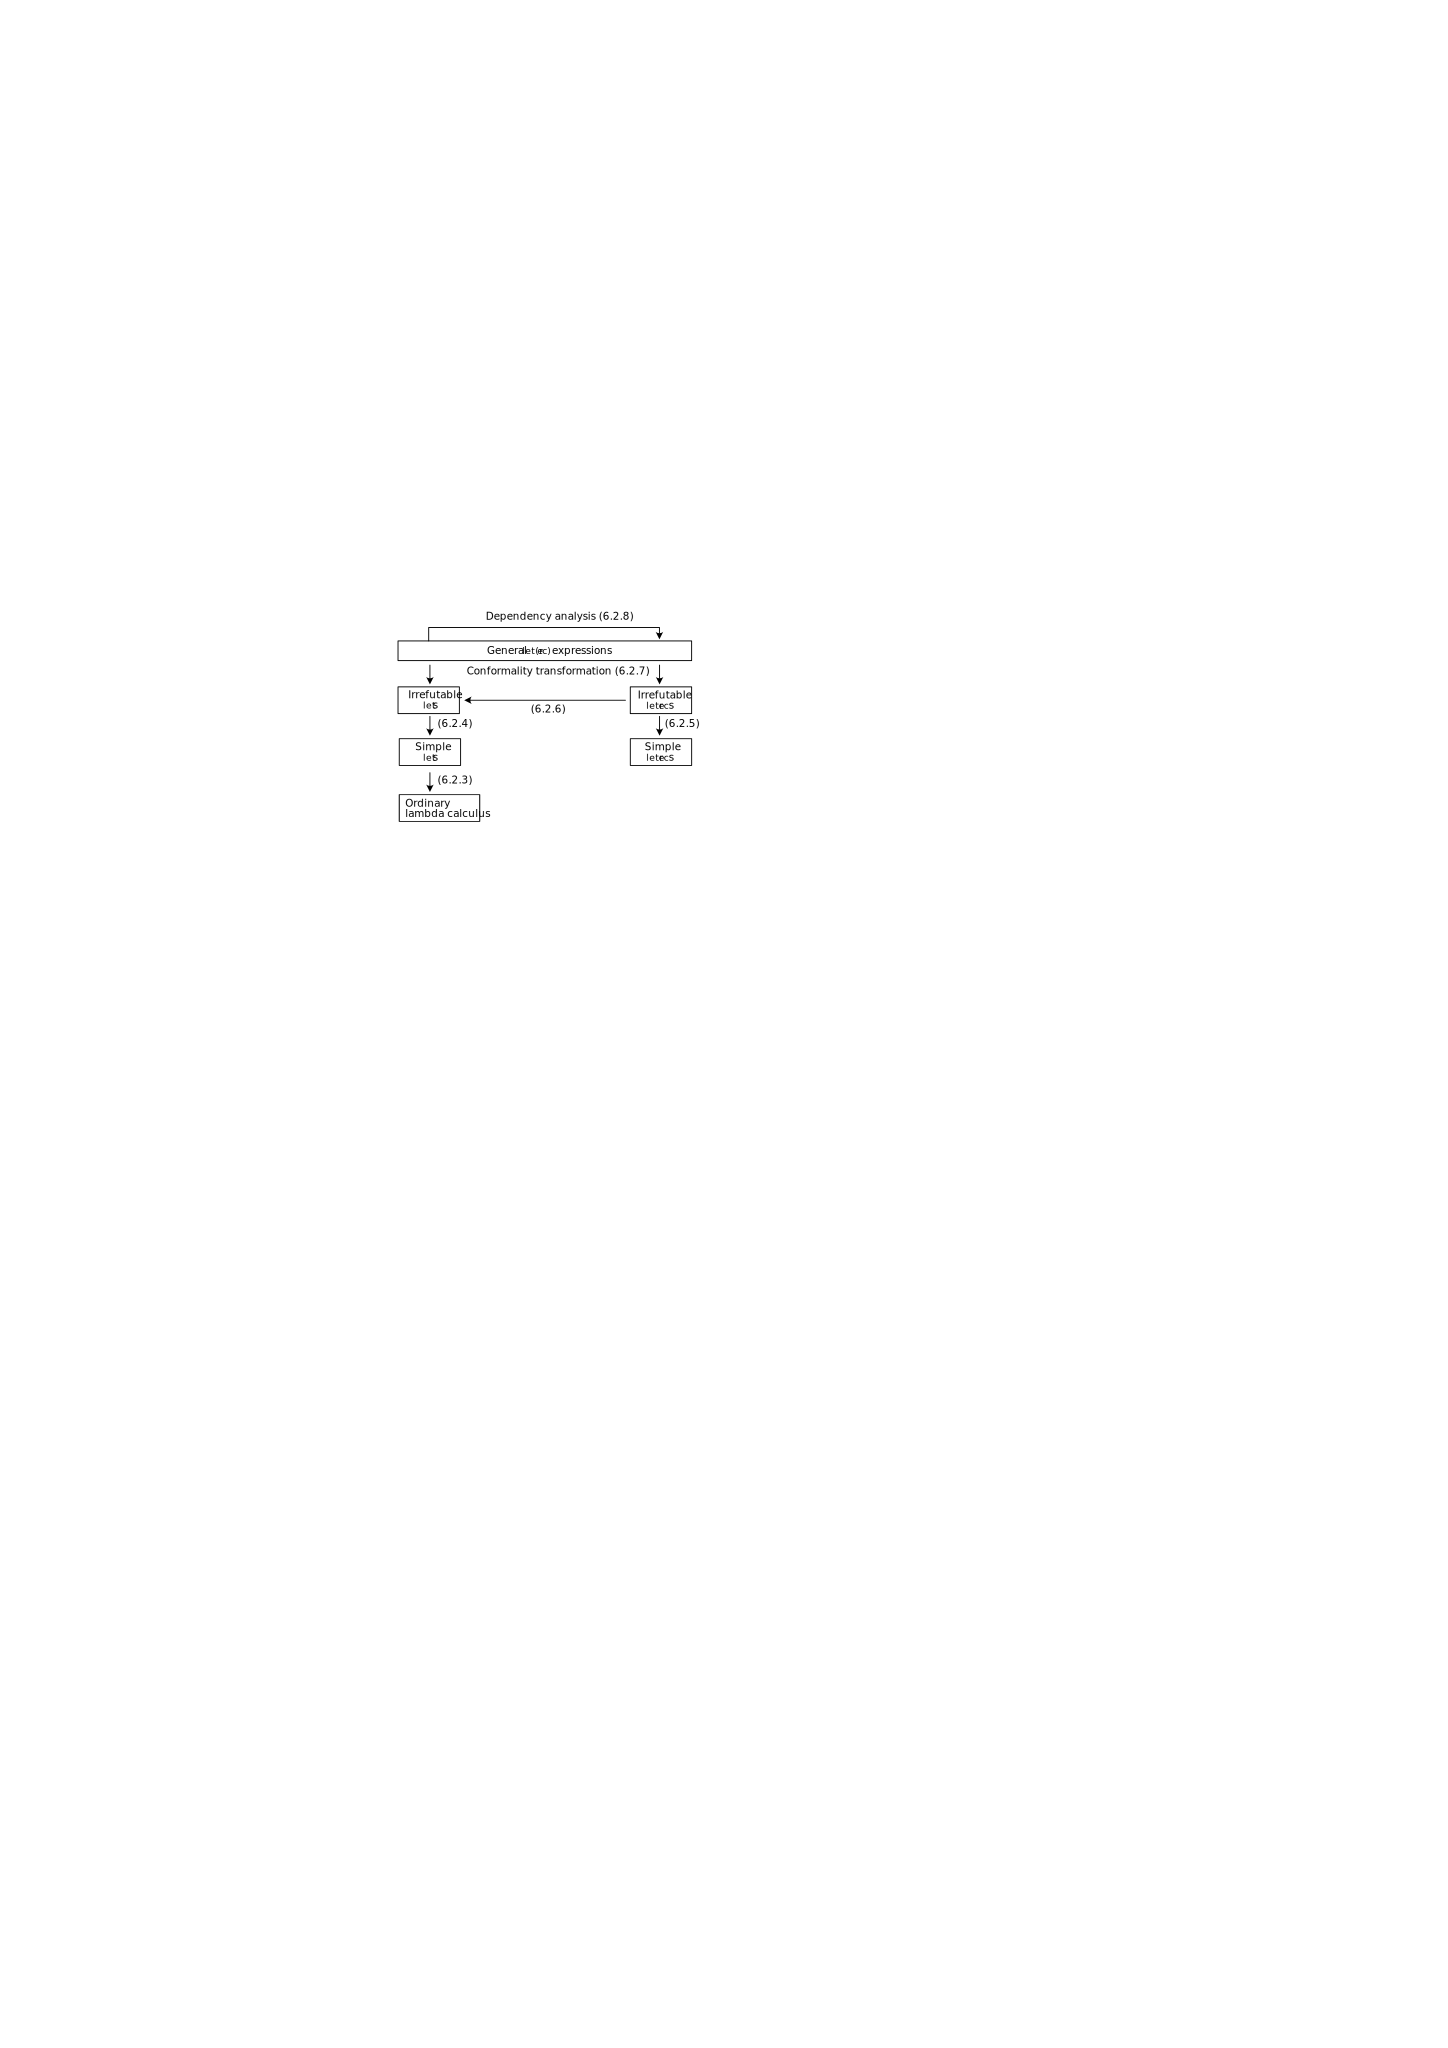
\includegraphics[width=0.96\textwidth]{chapters/Fig6_3}
			%                    \includesvg{chapters/Fig3_4}
			%                    \input{chapters/Fig3_4.tex}
			
		\end{minipage}%
		
	}%
	
	\caption{\textsf Map of \ml{let(rec)} transformations}
\end{figure}

\noindent Both possibilities are catered for by the transformations shown in Figure 6.3.

In what follows, when considering \ml{let}-expressions we assume that they
contain only one definition. This gives no loss of generality, since a \ml{let}-expression with multiple definitions is trivially equivalent to a nested set of
single-definition \ml{let}-expressions.

The following sections deal with the transformations depicted in Figure 6.3.

\subsection{Transforming Simple \ml{let}s into the Ordinary Lambda Calculus}

Once we have arrived at an expression in which all \ml{let}-expressions are simple,
it is easy to remove them altogether, using the transformation given in Section
3.2.1:

\plainbox{
\begin{mlcoded}
	let v = B in E $\equiv$ (\tlb{v}E) B
\end{mlcoded}
}
\noindent For example,
\begin{mlcoded}
	let x = 4 in (+ x 6) $\equiv$ (\tlb{x}+ x 6) 4
\end{mlcoded}

\subsection{Transforming Irrefutable \ml{let}s into Simple \ml{let}s}

Consider the case of an irrefutable \ml{let}-expression, of the form
\begin{mlcoded}
	let p = B in E
\end{mlcoded}
where \ml{p} is irrefutable. Since the pattern on the left-hand side of the definition
is irrefutable, it must either be a variable or a product pattern. In the former
case, there is nothing to do, since the \ml{let}-expression is already simple. In the
latter case, the \ml{let}-expression takes the form
\begin{mlcoded}
	let (t p$_1$ \ldots p$_r$) = B in E
\end{mlcoded}
where the \ml{p$_i$} are irrefutable patterns, and \ml{B} and \ml{E} are expressions. We can now
make the following transformation:

\plainbox{
\begin{mlcoded}
	\begin{tabular}{llll}
	let (t p$_1$ \ldots p$_r$) = B in E $\equiv$ \ &let &v =&\ B \\
		&in &(let &p$_1$ = SEL-t-1 v \\
		& & &\ldots \\
		& & &p$_r$ = SEL-t-r v \\
		& & \;\;in &E)
	\end{tabular}
\end{mlcoded}
where \ml{v} is a new variable that does not occur free in \ml{E}.
}

The \ml{p$_i$} are bound to selector functions applied to \ml{v}, which is in turn bound to
\ml{B}. Repeated application of this transformation will eliminate all non-simple
irrefutable \ml{let}-expressions.

To take an example, the expression
\begin{mlcoded}
	let (PAIR x y) = B in E
\end{mlcoded}
would be transformed to
\begin{mlcoded}
	\begin{tabular}{lll}
	let v = B in (&let &x = SEL-PAIR-1 v \\
		& &y = SEL-PAIR-2 v\\
		&in &E)
	\end{tabular}
\end{mlcoded}

Notice that if neither \ml{x} nor \ml{y} is evaluated in \ml{E}, then \ml{B} will not be evaluated
either, so the transformation implements lazy product-matching. Lazy
product-matching is just as much of an advantage here as it was in function
definitions. For example, we could recode the function \ml{firsts} from Section
4.3.5 in the following way:
\begin{mlcoded}
	\begin{tabular}{lll}
	firsts [\,] &= &(0, 0)\\
	firsts (x:xs) &= &(x, ev), \qquad odd x\\
	&= &(od, x), \qquad even x\\
	& &where\\
	& &(od, ev) = firsts xs
	\end{tabular}
\end{mlcoded}
We would expect this definition to behave just like that of Chapter 4, so that if
lazy product-matching is used for function definitions then it should also be
used for \ml{let}(\ml{rec})-expressions.

(Note: an alternative transformation would have been possible in this
section, namely:
\begin{mlcoded}
	let p = B in E = (\tlb{p}E) B
\end{mlcoded}
where \ml{p} is an irrefutable pattern. From a semantic point of view, this is
entirely equivalent to the transformation used above. However, for the
efficiency reasons outlined in Section 3.2.4, we prefer to stay in the world of
\ml{let}-expressions as long as possible; hence our choice.)

\subsection{Transforming Irrefutable \ml{letrec}s into Simple \ml{letrec}s}

The transformation from a letrec involving only irrefutable definitions into a
simple \ml{letrec} is very similar to that for \ml{let}-expressions:

\plainbox{
\begin{mlcoded}
	\begin{tabular}{llll}
	letrec &(t p$_1$ \ldots p$_r$) = B $\equiv$ &letrec &v = B \\
	&<other definitions> & & p$_1$ = SEL-t-1 v \\
	in E & & & $\cdots$\\
	&  & &	p$_r$ = SEL-t-r v \\
	& &	& <other definitions>\\
	& & in E & 
	\end{tabular}
\end{mlcoded}
where \ml{v} is a new variable that does not occur free in \ml{E} or \ml{B}.
}


All the transformed definitions must be in a single \ml{letrec}, to ensure that
variables in the patterns \ml{p$_i$} are in scope in \ml{B}. The `\ml{<other definitions>}' simply
takes into account the fact that the \ml{letrec} may contain multiple definitions, and
this transformation should be applied to each of them separately.